{
Vi vil nu give en intuitiv forklaring på, hvordan ovenstående metoder
sammensættes med det formål at trække regioner ud af et billede.
Regioner trækkes ud i forhold til et snit i billedet, således at vi kun
finder regioner inden for margin relevant for dette snit. Vi går gennem
fire skridt, når vi trækker regioner ud, hvoraf de tre første kan
betragtes som forberedelse af billedet inden den endelige segmentering med floodfill:

\begin{enumerate}
    \item \textbf{Kantdetektion}\\
Først finder vi kanter i billedet --- de skal bruges kanterne senere
skridt. Vi bruger parametrene $(72, 180)$ og resultatet kan ses i figur
\ref{sammen_kanter}.

\item \textbf{Sløring}\\
Billedet sløres, således at vi senere kan male større regioner med
floodfill. Vi bruger simpel sløring med en $3\times3$ foldningsmatrix.
Det slørede billede ses i figur \ref{sammen_slor}, men når
billedet er skaleret ned, ses sløringen ikke så godt.

\item \textbf{Fremhævelse af kanter}\\
Når billedet er blevet sløret, har vi ikke så gode kanter længere. Vi
tager nu de originale kanter og lægger dem oven på billedet, således at
kanterne bevares. Billedet med fremhævede kanter kan ses i figur
\ref{sammen_frem_kant}.

\item \textbf{Udtrækning}\\
Vi har nu et sløret billede, men med de originale kanter fremhævet.
Dette billede segmenteres nu ved hjælp af floodfill. De originale kanter
bruges i dette skridt til at fortælle floodfill-metoden, hvor nye
regioner starter. Vi bruger således floodfill ned langs et snit i
billedet og bruger en ny farve, når vi passerer en kant i det originale
billede.
\end{enumerate}

I figur \ref{sammen_floodfill} bruger vi kun floodfill-metoden på
snittet. Derved fanger vi ikke regioner, som ligger \emph{tæt} på
snittet. Vi tager derfor vores margin og bruger også floodfill på dette.
Hvis vi betragter et vertikalt snit, bruges floodfill altså tre gange;
én gang på det venstre margin, én gang på snittet og endelig én gang på
det højre margin. Vi fanger derved de regioner, som befinder sig inden
for vores margin. Dette ses i figur \ref{sammen_floodfill_margen}.

\begin{figure}[!p]
    \centering
    \subfloat[Kantdetektion]{
        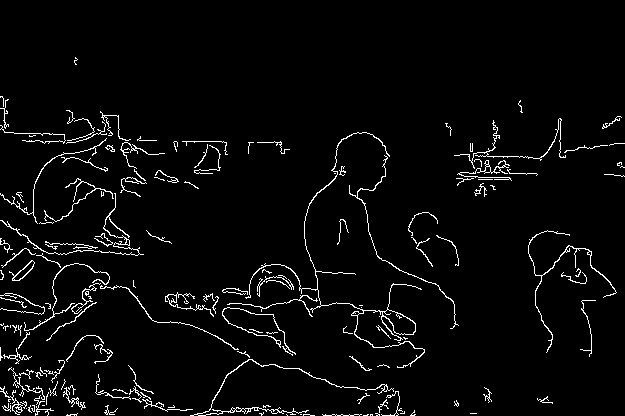
\includegraphics[angle=0,width=0.45\textwidth]{afsnit/vores_implementation/billeder/sammensaetning/kanter}
        \label{sammen_kanter}}\hspace{1em}
    \subfloat[Sløring]{
        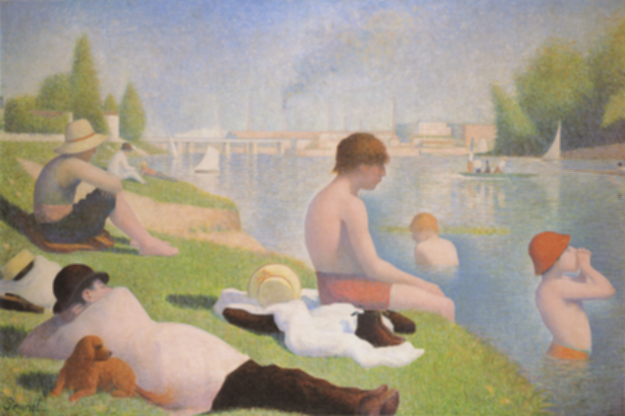
\includegraphics[angle=0,width=0.45\textwidth]{afsnit/vores_implementation/billeder/sammensaetning/sloering}
        \label{sammen_slor}}\\
    \subfloat[Fremhævelse af kanter]{
        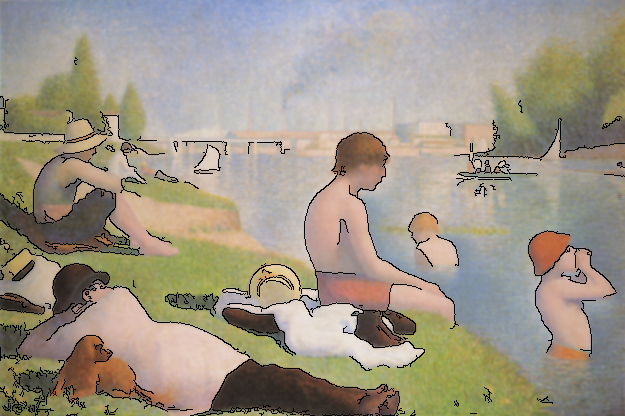
\includegraphics[angle=0,width=0.45\textwidth]{afsnit/vores_implementation/billeder/sammensaetning/fremhaevet}
        \label{sammen_frem_kant}}\hspace{1em}
    \subfloat[Udtrækning af regioner på snittet]{
        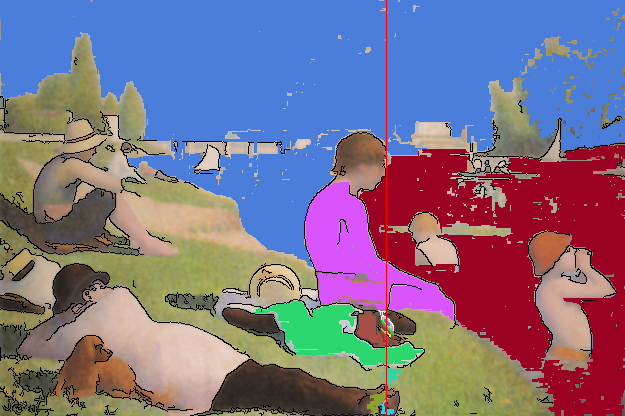
\includegraphics[angle=0,width=0.45\textwidth]{afsnit/vores_implementation/billeder/sammensaetning/combined_no_margin}
        \label{sammen_floodfill}}\\
    \subfloat[Udtrækning af regioner inden for margin]{
        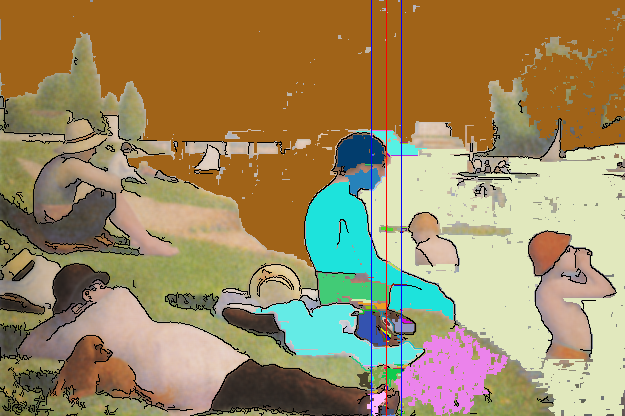
\includegraphics[angle=0,width=0.8\textwidth]{afsnit/vores_implementation/billeder/sammensaetning/combined_margin}
        \label{sammen_floodfill_margen}}
    \caption[]{Udtrækning af regioner i forhold til et snit.}
    \label{sammensaetning}
\end{figure}

\subsubsection{Vurdering}
Vi har her præsenteret grundprincipperne i vores metode til udtrækning
af regioner. Metoden er præsenteret med henblik på udtrækning omkring
det gyldne snit, men ethvert andet snit i billedet kan bruges. Det skal
bemærkes, at den samme region godt kan trækkes ud af flere snit. Når
regionerne, der er relevante for et snit, er trukket ud af billedet, kan
de vurderes efter den simple fremgangsmåde givet i afsnit
\ref{section_naiv}.

I kapitel \ref{chap_implementation} vil vi komme ind på de tekniske
begrænsninger og problemer med denne fremgangsmåde, som vedrører den
egentlige implementation af metoden.

}

% vim: set tw=72 spell spelllang=da:
